\chapter{\textit{Reporting}}


%====> Lien intéressant pour tous (office national de statistiques pour les UK, avec un tas de diagrammes complets et intéressants) : http://www.ons.gov.uk

%\section{Cube patate}


%Le lien ci-dessous peut être utile : graphique d'évolution des conditions sanitaires (health) pour les différentes classes de population par famille de cluster

%\begin{verbatim}
%http://www.google.fr/url?sa=t&rct=j&q=&esrc=s&source=web&cd=4&ved=0CEoQFjAD&url=http%3A%2F%2Fwww.ons.gov.uk%2Fons%2Fguide-method%2Fgeography%2Fproducts%2Farea-classifications%2Fns-area-classifications%2Findex%2Fcluster-summaries%2Fhealth-areas%2Fprospering-uk.pdf&ei=LodSU-raKqiZ0QXjr4CwDw&usg=AFQjCNESWJHRf0se4ScTkOhLLWBMoYvW3g&sig2=PxLbntsqK0DGj7pG3Us-Kw&bvm=bv.65058239,d.d2k
%\end{verbatim}

\subsection{Troubles mentaux, et évolution de leur prise en charge}

    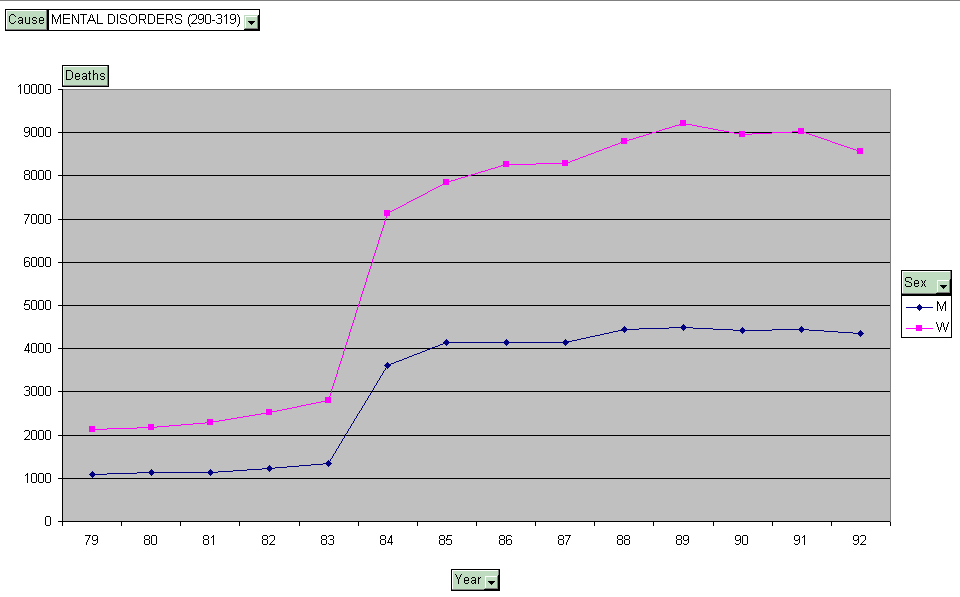
\includegraphics[scale=0.5]{images/mental_disorder.png}

    Une cause de mort a attiré notre attention plus que les autres~: les ``mental disorder''. En plus de présenter une grande disparité
    entre morts chez les hommes et les femmes, le nombre morts causées par ces troubles a drastiquement augmenté en 1983.

    Nous avons essayé de chercher des signes d'une augmentation aussi drastique des morts chez les autres causes, en vain. Il était donc
    clair que cette augmentation était bien spécifique aux \textit{troubles mentaux}.

    Nous sommes donc allés chercher les événements marquants s'étant produits en Grande-Bretagne autour de 1983, et quelques recherches
    et articles plus tard, nous avons isolé la cause à l'origine de cette hausse : le \href{en.wikipedia.org/wiki/Mental_Health_Act_1983‎}{Mental Health Act of 1983}.

    Cet acte parlementaire a introduit une nouvelle classification des \textit{troubles mentaux} et un traitement

\subsection{Morts néonatales et nouveaux certificats de décès}

    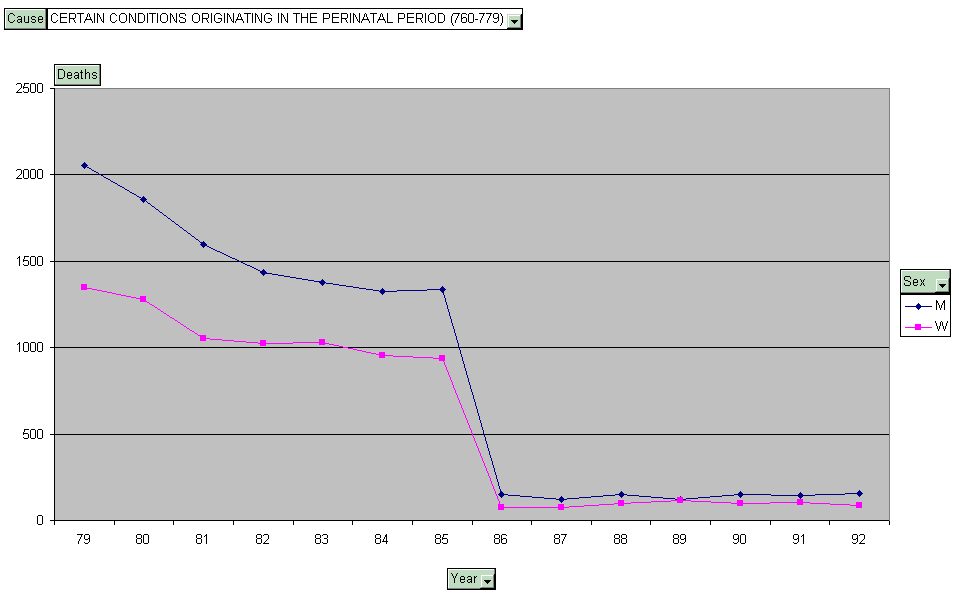
\includegraphics[scale=0.5]{images/perinatal.png}

    Blah blah.

\subsection{Maladies musculo-squelettique}

    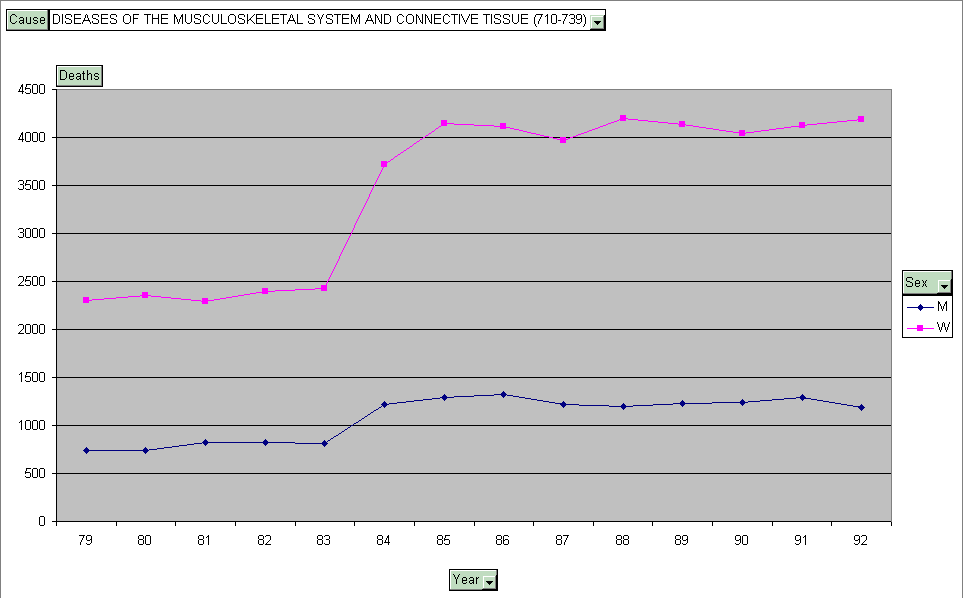
\includegraphics[scale=0.5]{images/muscoskeletal.png}

    Blah blah.

\pagebreak


\section{Cube Population}
\subsection{Évolution de la population au cours du temps}
\begin{figure}[h!]
    \centering
    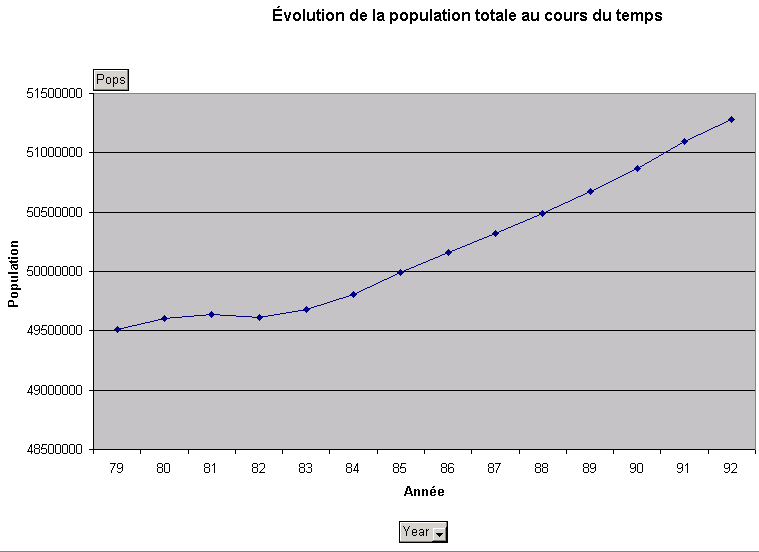
\includegraphics[width=\linewidth]{images/pop/evolutionPopulation.png}
\end{figure}

Le graphique précédent illustre la croissange démographique générale des Royaumes Unis entre 1972 et 1992. Cette courbe est en accord avec celles d'autres pays occidentaux à la même époque, la croissance démographique étant ici linéaire et en faible progression.

On notera que les relevés de population précédant l'année 1981 diffèrent de par la technique de comptage effectué. Avant cette date, les touristes présents aux Royaumes Unis étaient comptabilisés dans les données de population, alors que les résidents qui étaient hors du territoire à la date de rencencement ne l'étaient pas. À compter de 1981, les touristes n'étant plus comptés, et les résidents l'étant, ceci explique l'allure légèrement décroissante de la courbe entre 1981 et 1982.

On observe alors une population résidente d'environ 49 650 000 personnes en 1982, ce chiffre culminant à 51 300 000 personnes en 1992, soit une croissance d'environ 3.32\% (+1 650 000 résidents) en 10 ans.
\pagebreak


\subsection{Évolution de la répartition hommes / femmes au cours du temps}
\begin{figure}[h!]
    \centering
    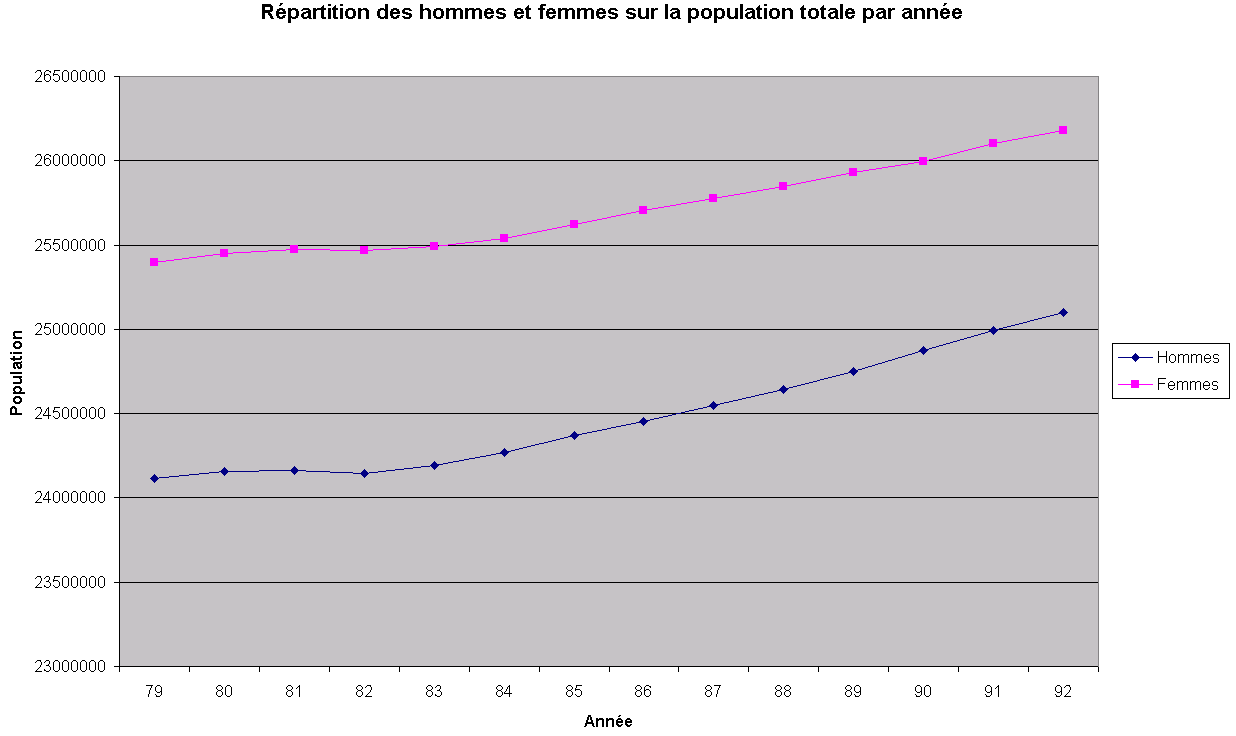
\includegraphics[width=\linewidth]{images/pop/repartitionHF.png}
\end{figure}

On peut ici observer que la répartition hommes / femmes est restée constante au cours du temps, l'allure d'une courbe épousant aisément celle de l'autre.

On dénote près de 24.2 millions d'hommes et 25.5 millions de femmes aux Royaumes Unis en 1982 contre respectivement 25.1 et 26.2 millions en 1991.

Ceci représente une croissance de 3.72\% (+0.9 millions) chez les hommes et 2.75\% (+0.7 millions) chez les femmes.

La croissance démographique est donc plus grande chez les hommes que chez les femmes.
\pagebreak


\subsection{Répartition de la population par classes d'âge en 1992}
\begin{figure}[h!]
    \centering
    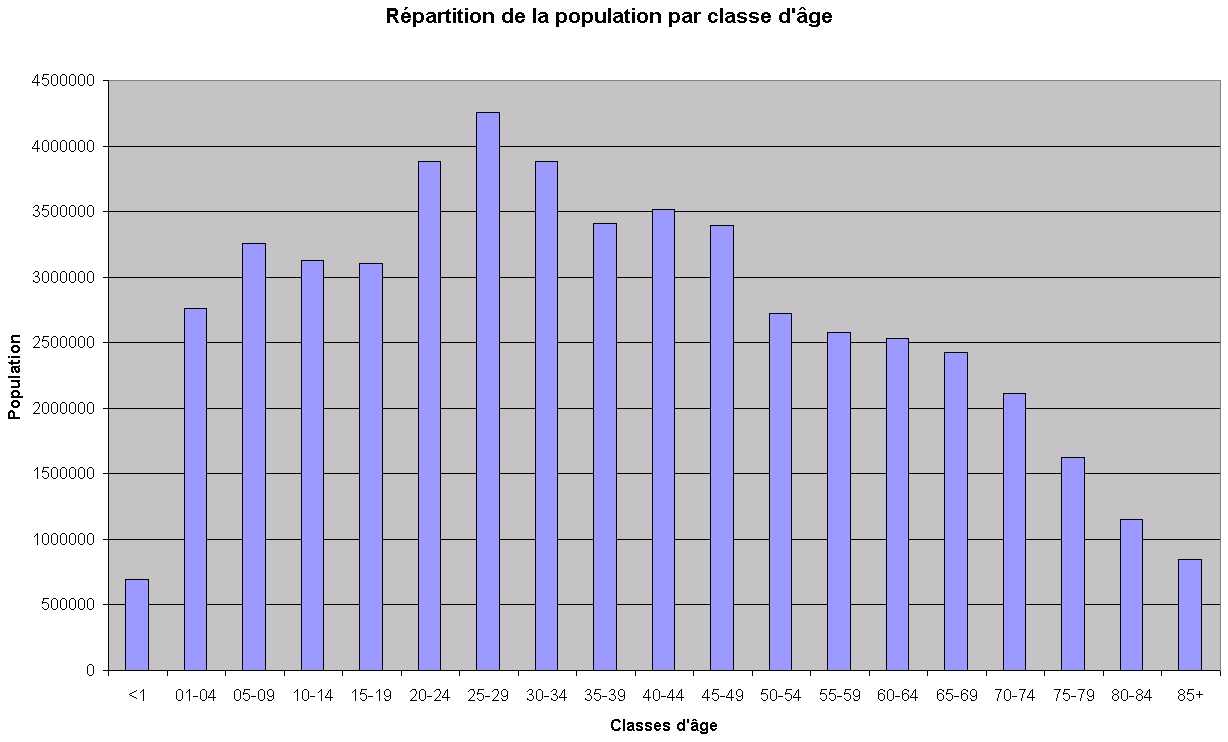
\includegraphics[width=\linewidth]{images/pop/pyramideAges.png}
\end{figure}

En accord avec les répartitions par classes d'âges des pays européens à cette époque, le graphique ci-dessus illustre une pyramide des âges tout à fait standard pour un pays développé.
\pagebreak


\subsection{Répartition de la population}

\begin{figure}[h!]
    \centering
    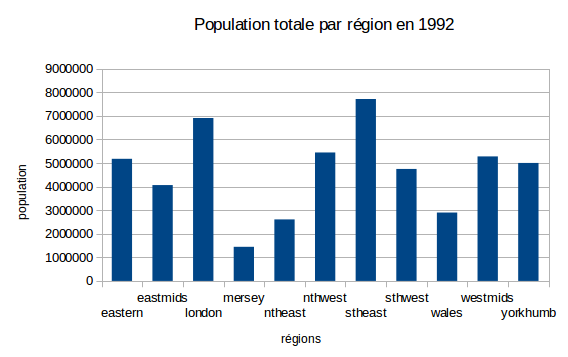
\includegraphics[width=\linewidth]{images/pop/popRegion.png}
\end{figure}

\begin{figure}[h!]
    \centering
    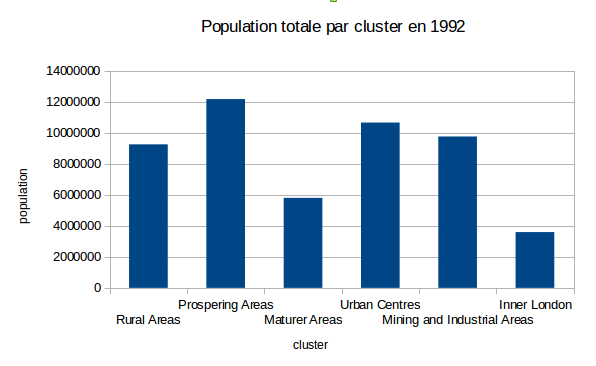
\includegraphics[width=\linewidth]{images/pop/popCluster.png}
\end{figure}

Grâce à ces histogrammes, nous pouvons observer la répartition de la population aux UK, et remarquer encore une fois le lien entre économie et population. Les régions propsères regroupent un nombre élevé de personnes. Mais il faut noter que nous n'avons ici pas connaissance de la taille des différents clusters. Or, si pour les régions les tailles sont à peu près semblables, ce n'est pas le cas des clusters, qui parfois couvrent bien plus de surface que d'autres. Pour les régions, le merseyside est une petite région face aux autres, il est donc normal d'observer un faible nombre de personnes. Mais on reste tout de même dans une région économiquement souffrante dans les années 80 donc n'étant pas forcémment des plus peuplée en 1992.
Les régions du Sud de de Londres regroupent un grand nombre de population du fait de leur situation géographique plus proche du reste de l'europe et dans un climat plus agréable que le Nord.

\pagebreak


\subsection{Déplacements de population par région}
\begin{figure}[h!]
    \centering
    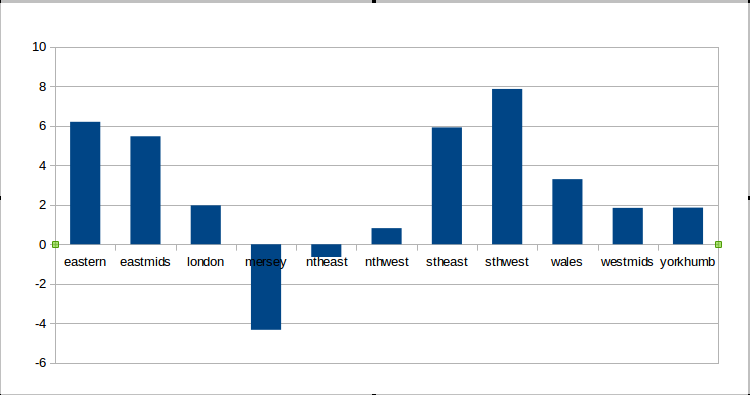
\includegraphics[width=\linewidth]{images/pop/deltaPopRegions.png}
\end{figure}

Dans cet histogramme, nous pouvons observer deux faits notables : le premier, est la chute assez importante (plus de 4\%) de population dans le merseyside. Il semblerait qu'un fait politique/économique ait entrainé un déplacement de population en dehors de la région du mersey. Après renseignement, le merseyside a subit de forts problèmes économiques dans les années 80, ce qui expliquerait une volonté de la population de fuir cette région, au profit des autres qui, second fait notable, connaissent quasimment toutes une augmentation significative de leur population, avec en tête le southwest, région ouverte au reste de l'europe et plutôt propice à attirer la population.



\pagebreak


\subsection{Déplacements de population par famille de clusters}

\begin{figure}[h!]
    \centering
    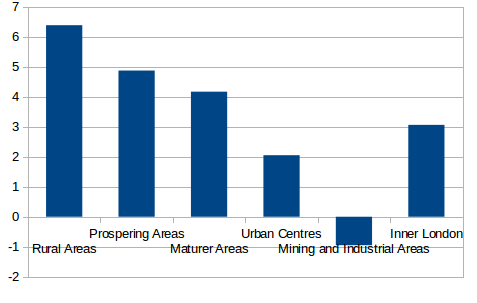
\includegraphics[width=\linewidth]{images/pop/deltaPopFamilleCluster.png}
\end{figure}

On observe ici les effets d'une exode rurale toujours présente au cours des dernières années, la population urbaine tendant à retourner au sein du milieu rural. En effet, si la population tend à croître dans les milieux urbains (+220 000 personnes pour les centres urbains, et +90 000 pour le centre londonien) et ruraux (+600 000 personnes), sa croissance est bien plus forte pour les zones rurales, dénotant un déplacement de population certain au cours des 10 années d'étude.

Ce déplacement est d'autant plus visible au sein des milieux miniers et industriels, les zones rattachées au secteur secondaire observant une diminution de près de 130 000 personnes.
\pagebreak

popc